% g-2 Introduction
\chapter {Introduction} \label{ch:intro}
In particle physics, \gmtwo of the muon, and \gmtwo in general, is an important and deep probe into the Standard Model (SM). The g-factor, $g$, represents the coupling strength of a particle to the type of helicity flipping transitions mediated by magnetic fields, and the ``$\hbox{--}2$'' portion denotes the subtraction of the expected value of the g-factor without quantum field effects, leaving only the anomalous magnetic moment.

\begin{equation}
\label{eqn:a-lepton}
a_{\ell} \equiv \Big(\frac{g\hbox{--}2}{2} \Big)_\ell
\end{equation}

\noindent
The two values, $a$ and \gmtwo, are used interchangeably even though are technically different by a factor of two.  The quantity acts as both a seed and a scythe for models which extend \tsm.  Contributions to the quantity arise from the full gamut of fundamental interactions and constants of the universe in the SM: Quantum Electrodynamics (QED), Electro-Weak Interactions (EW), and Quantum Chromodynamics (QCD) all playing important roles.  Precision measurements of \gmtwo are somewhat unique in this regard, and perhaps for that reason, experimentalists have been fascinated by \gmtwo for many years.

In the subsequence sections, the \mugmtwo is fully introduced.  The discussion starts with simple essential properties of the quantity.  Then, proceeds lay down the science impetus for performing experiment to measure it.  Next, a short regaling tells of the history behind \gmtwo experiments.  And, finally an overview of the theoretical calculation against which the measurement compares its results.

\section{Magnetic Moment Fundamentals} \label{sec:mag-moment-fundamentals}

A thorough understanding of muon \gmtwo begins with classical model for a magnetic moment.  An entity attains a magnetic moment when the object has net correlation between electric charge and angular momentum.  Equation \ref{eqn:magnetic-moment-integral} shows the calculation for such a correlation \note{this might not be exactly what I want}.

\begin{equation}
\label{eqn:magnetic-moment-integral}
\mu = \int \vec{r} \times \vec{j} \,dV
\end{equation}

\noindent
The angular momentum can be physical, $\vec{L}$, or intrinsic spin, $\vec{S}$, so the equation holds, classically at least, for volumes and point-like particles with spin. The caveat is that there is a proportionality constant, the g-factor, which must be included in the spin calculation of the equation giving rise to equation \ref{eqn:spin-magnetic-moment} for magnetic moments that arise due to spin.

\begin{equation}
\label{eqn:spin-magnetic-moment}
\vec{\mu} = g \frac{e}{2m}\vec{S}
\end{equation}

The g-factor can vary extensively between different particles.  The proton g-factor is 5.5, and the neutron, which naively should not even have a magnetic moment due to a lack of net charge, has a g-factor of -3.8 \cite{codata}.  For point-like particles the g-factor was calculated to be exactly 2 by using the Dirac Equation.  Initial experiments measuring electron and muon \gmtwo were consistent with the calculation that $g \equiv 2$.  Discrepancies did not arise for several years, and that discussion is contained in \ref{sec:history-expt} rather than here.  The short of it is that quantum interactions with the the vacuum shift the value of $g$ at the \SI{0.1}{\percent} level.

Intuitively, a magnetic moment is similar to macro-scale magnet that all children are all familiar with.  One of the important behaviors exhibited is a tendency to anti-align with external magnetic fields.  Such macro behavior is useful in compasses to align with the Earth's magnetic North Pole and seen with bar magnets where oppositive ends attract.  The behavior holds true in the micro as well, and this behavior turns out to be crucial in pulsed nuclear magnetic resonance (pNMR) measurements.  Precession is another important behavior arising from a non-zero magnetic moment.  A magnetic field orthogonal to the particle's magnetic moment causes the magnetic moment vector to rotate in plane orthogonal as prescribed by equation \ref{eqn:classical-precession}. Without spin precession, an entirely new method for measuring $g$ would have to be conceived let alone measuring \gmtwo \note{do I mean this?}.

\begin{equation}
\label{eqn:classical-precession}
\omega = \frac{\mu B}{2 m}
\end{equation}

\section{Motivation}

There are two major questions that need answers to motivate the muon \gmtwo experiment.  The first equations is: "Why measure the anomalous magnetic moment?", and the second question is: "Why use muons?".

To the first charge, there are many appropriate replies.  One answer is that it is a simple measurement in principle.  The experimenters need a polarized volume of particles, an external vertical magnetic field, and a technique to determine the spin direction. Another, more phenomenological answer is that \gmtwo serves as a multi-faceted probe into quantum field theories in general and the Standard Model in particular.  Calculating the value for \gmtwo requires careful consideration of effects arising in Quantum Electrodynamics, Electro-Weak Theory, and Quantum Chromodynamics.  It nearly traverses the entirety of the Standard Model.

And, to the second question, there are physics considerations and practical considerations.  The physics consideration weighs in with the desire for sensitivity to the intricacies of the Standard Model.  The more intricate, higher order interactions general come into the playing field with mass suppression terms, $\propto (\frac{m}{M})^2$, or possibly an a higher power than 2.  The relative mass ratio between the electron and the muon enhance these terms by a factor of $(\frac{105.66}{0.511})^2 \approx 43,000$ \cite{the-muon-g-2}!  The preceding argument begs the question though: "Why not use the $\tau$?".  The answer is really a practical consideration; the ephemeral $\tau$ has a lifetime of only \SI{0.29}{\femto\second} compared to \SI{2.2}{\micro\second} for $\mu$ \cite{codata}.  While the $\tau$ particle is appealing if a significant enough Lorentz boost could be achieved, an experiment using $\tau$ particles is simply not practical with current technology.

\subsection{Statistical Tension}

The muon \gmtwo has been measured many times over the years.  And, throughout it has been a constant probe of the Standard Model and beyond.  The experiment value has come along from a modest start when it agreed with the classical calculation of $g\equiv2$ \todo{cite initial expt} to gradually highlighting a \SI{3}{\sigma} deviation from Standard Model predictions.  The experiments are discussed further in section \ref{sec:history-expt}.  Theoretical calculations are similarly discussed more in section \ref{sec:theory}.  The measured and calculated \mugmtwo values have kept similar pace over the year, no doubt due to pushing on one front inspiring pushes on the other, and the progression of the value can be seen in figure \ref{fig:intro-historical-values}.  The path of theory and experiment split over the years to arrive at the current values which exhibit a \SI{3}{\sigma} statistical tension.  The large persistent discrepency is seen as a likely indication of new physics from beyond \tsm.

\begin{figure}
\label{fig:intro-historical-values}
\includegraphics[width=0.9\linewidth]{fig/intro-historical-values}
\caption{The progression of theoretical and experimental values for \mugmtwo over the years.  A clear divergence in each can be seen as the precision for each increases.  The latest inputs place the statistical tension between theory and experiment at about \SI{3}{\sigma}.}
\todo{take notes and add more theory values, add references}
\end{figure}

\section{History of Experiment} \label{sec:history-expt}

The notion that $g \ne 2$ had to be reconciled with experiment as measurement precision progressed and statistical tensions arose with the values predicted by theory.  Deviations from a pure Dirac particle were first observed in hyperfine splitting measurements of several different nuclei \todo{reference}.  The measured deviations were not statistically significant until Kusch and Foley measured the atomic spectra of several nuclei in 1947 \cite{kusch-foley}.  The theory community quickly resolved the discrepancy with a now standard QED calculation of the lowest order self-interaction for leptons emitting and reabsorbing photons, see figure \ref{fig:schwinger-diagram}.  The Schwinger term, coined after Julian Schwinger, brought experiment and theory back into good agreement.  It served as an early triumph of QED. 

\begin{figure}
\label{fig:schwinger-diagram}
\centering
\includegraphics[width=0.2\linewidth]{fig/schwinger-diagram}
\caption{The Feynman diagram for the so-called Schwinger term. The propogating lepton radiates a photon, interacts with the magnetic field via a disconnected photon and re-absorbes the radiated photon.  The contribution to \gmtwo from the interaction is $\frac{\alpha}{2\pi}$.}
\end{figure}

\subsection{Parity Violation}
The first direct measurement of the anomalous magnetic moment, \gmtwo, came later, and the muon \gmtwo much later.  The first measurement of $g_e$ happened in 1953 by H. R. Crane, et al. \todo{can't find pdf of paper}.  Subsequent theoretical calculations and supporting experimental measurements established $g_e$ as the most precisely predicted and measured quantity of QED.  As for measuring $g_\mu$, no one knew how to properly control the polarization of the muons, that is until parity violation of the Weak interaction came to light.  With parity violation baked into the Weak interactions, researchers quickly realized that pions would decay into muons polarized along the beam direction.  

\subsection{CERN-I}
Building off the Weak parity revelation, researchers measured $g_\mu$ for the first time.  In 1960 Columbia personnel measured the quantity to $5\%$, and not long after a more precise measurement came out of CERN and eclipsed it.  The experiment worked by injecting relatively low energy, \SI{83}{\MeV}, muons into a long, narrow magnetic trap where the polarized muons would undergo both cyclotron motion and lateral drift, see figure \ref{fig:cern-i-diagram}. At the opposite end of the magnet, the muons were ejected, tagged for storage time, and stopped where the momentum direction of electron was recorded as recorded as either forward or backward.  Using this technique CERN scientists were able to achieve a precision of $0.4\%$, absolutely phenomenal for the time \cite{cern-i}.  A deviation of $1.6\,\sigma$ was present at the achieved precision.

\begin{figure}
\centering
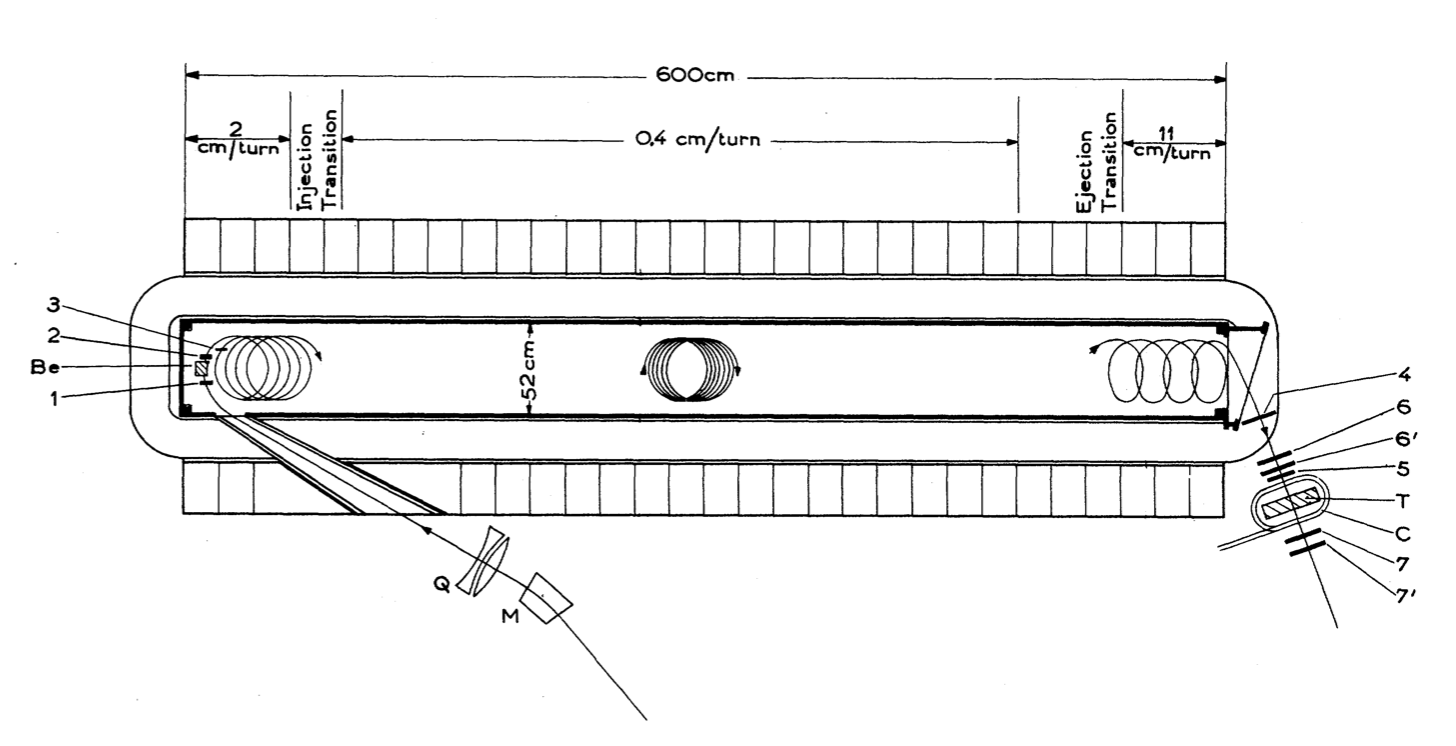
\includegraphics[width=0.9\linewidth]{fig/cern-i-diagram.png}
\label{fig:cern-i-diagram}
\caption{A diagram of the experimental setup in the first muon \gmtwo experiment at CERN. The muons enter from the lower left, go through the energy moderator to put the cyclotron radius at 19cm, drift and circles toward the ejection side of the magnetic, escape from the the magnet, stop in the fiducial block, and decay into an electron with momentum correlated to the spin direction.}
\end{figure}

\subsection{CERN-II}
The second iteration of \mugmtwo at CERN improved vastly over the first.  CERN-II was the first \mugmtwo to use the now familiar storage ring.  In order to store muons, the experiment injected a beam of protons which hit a pion production target.  A slice of the pion production phase space matched the momentum acceptance of the ring well enough to remain for several revolutions. And, some fraction of the muons produced from pion decay were mostly forward decays that lost a bit of energy and matched the ring's momentum acceptance.  The decay electrons curled inward to electron counting detectors at a rate modulated at \gmtwo frequency.  The injected muons had a relativistic $\gamma$ of 12 which allowed the researchers to measure muon spin precession for more than 130 $\mu s$ which led to determination of $a_\mu$ to \ppm{270} \cite{47y-muon-g-2}.

\subsection{CERN-III}
The final CERN muon \gmtwo experiment ran from 1969 to 1976.  A major innovation introduced in CERN-III was use of the so-called "magic" momentum. Observe equation \ref{eqn:full-omega-a}, the expression for spin precession in electromagnetic fields for a relativistic muon.

\begin{equation}
\label{eqn:full-omega-a}
\omega^\prime_a = \omega_a[1 + (1 - 1 / a \beta^2 \gamma^2)(\beta E_r / B)]
\end{equation}

\noindent A muon beam at a very specific momentum, \pmagic, cancels the effects of of radial electric fields which allows electrostatic focusing to be used on the muon beam instead of magnetic gradient focusing.  Another major innovation for the third CERN experiment was the use of pion injection instead of proton injection.  The measurement techniques of CERN-III were similar to CERN-II.  With the achieved improvements, the CERN team was able to drive down the uncertainty on $a_\mu$ to \ppm{7}, nearly a 40-fold improvement \cite{47-years}!

\subsection{E821 at BNL}
The most precise \mugmtwo experiment to date, took place at Brookhaven National Laboratory (BNL). The experiment, E821 as it is labeled in high energy physics ledgers, pushed precision muon phyiscs to the next level.  The precision goals for E821 demanded a 400-fold increase in statistics over its predecessor.  In order to accommodate the necessesited higher rates, the decay electron measurement platform was separated into 24 individual calorimeters.  Another critical improvement in the experiment, E821 injected muons rather than pions, or protons.  Muon injection provided a cleaner data earlier in each fill.  The experiment design also focused on improving the homogeneity of the magnetic storage field.  The aperture of the storage region was increased to facilitate a more uniform field across the muon storage volume.  Field measurement was also improved by implementing both a suite of fixed probes always monitoring magnetic field drift outside of the storage region and a trolley outfitted with an array of 17 probes to measure the field in the storage volume periodically.  In the end, the experiment nearly achieved the initial goal of 350 ppb uncertainty on $a_\mu$, actually reaching 540 ppb uncertainty\cite{e821-prd}.

The E821 \gmtwo result was at odds with theoretical calculations.  Depending on which theoretical models were employed, the measurement was somewhere around $3.3\sigma - 3.6\sigma$ away from theoretical prediction, a statistical tension.  The tension remained in subsequent years, inspiring a new iteration of the \mugmtwo experiment at Fermi National Accelerator Laboratory (FNAL). The experiment, E989, reuses the storage ring, superconducting coils, and various components from the BNL experiment.  The goal of E989 is an overall uncertainty of 140 ppb, likely pushing the tension to discovery levels, i.e., \SI{5}{\sigma}. Additionally, a sister experiment is underway at J-PARC as a completely independent measurement of \mugmtwo with similar sensitivity as the BNL experiment.  In a parallel effort, theoretical particle physics researchers have been pushing the precision of calculations to match pace with experiment \todo{references}.

\section{Theory Contributions} \label{sec:theory}

The theoretical contributions to muon \gmtwo come from all corners of particle physics.  The typical diagonalization of the contributions breaks them into QED, Weak, and Strong. The relative sizes of the contributions are displayed in figure \ref{fig:sm-contributions} and layed out in equation \ref{eqn:sm-contributions}. The Electro-Weak contributions are well modeled, and theoretical progress involves calculating increasingly intricate Feynman diagrams.  The Strong contributions are trickier and represent a larger challenge to the theory community.  The theory community as set a similar precision goal as the E989 collaboration, \SI{140}{ppb}, following a similar time frame, around 2020 \cite{e989-tdr}.

\begin{figure}
\includegraphics[width=0.9\linewidth]{fig/SM-contributions.pdf}
\label{fig:sm-contributions}
\caption{The spectrum of theoretical contributions to muon \gmtwo.}
\end{figure}

\begin{equation}
\label{eqn:sm-contributions}
a_\mu = a_{_{QED}} + a_{_{EW}} + a_{_{QCD-HVP}} + a_{_{QCD-LBL}}
\end{equation}

\subsection{QED Effects} \label{s-sec:theory-qed}

The correction from QED interactions is by far the lionshare of $a_\mu$.  Feynman diagrams provide a convenvient method to intuit some of the relevant effects.  And, there are a few different types of interaction diagrams that the QED effects can be divided into.  One type of diagram is of the radiative correction type, shown in figure \ref{fig:qed-feynman-diagrams} (1\hbox{--}4).  These diagrams involve emission and recapture of a photon(s) while the particle is in flight.  Another common type of diagram is vacuum polarization interactions, shown in figure \ref{fig:qed-feynman-diagrams} (5\hbox{--}6), which resemble radiative correction with the offshell photon going through pair production and annihilation along its path.

\begin{figure}
\label{fig:qed-feynman-diagrams}
\includegraphics[width=0.9\linewidth]{fig/qed-feynman-diagrams}
\caption{Several examples of QED interactions illustrated as Feynman diagrams.  The first four constitute radiative corrections, and the last two are termed vacuum polarization effects. \note{came from John Donaghue's UMass page, reference or generate my own diagrams}}
\end{figure}

The QED corrections constitute over 99\% of the total anomalous magnetic moment and the bulk of that arises from the lowest order term.  A natural way to represent QED corrections is through a power series in the QED coupling constant, $\alpha_{_{QED}}$.

\begin{equation}
\label{eqn:qed-correction-series}
a_{_{QED}} = \sum_n{A_n\frac{\alpha_{_{QED}}}{\pi}^n}
\end{equation}

\noindent
The first term in the series is solely the leptonically universal Schwinger term, $\delta a_{Schwinger} = \frac{\alpha_{QED}}{\pi}$.  In terms of the measured value of \gmtwo of the electron, the Schwinger term is $100.134\%$ of the measured value. And for the muon \gmtwo, the lowest order term is a slightly larger fraction of the total at $99.59\%$ \cite{codata}.  In both cases though, the Schwinger term absolute dominates the corrections.

\begin{align*}
a_{e}   & = 115 965 218.091(26) \times 10^{-11} \\
a_{\mu} & = 116 592 080(63) \times 10^{-11} \\
a_{_{Schwinger}} & = 116 120 635.555(27) \times 10^{-11}
\end{align*}

Investigation of the limits for an expression of the vertex is another useful window in the next order of QED effects which includes radiative corrections and vacuum polarization effects.  First, consider the case in which the radiated particles are light compared to the muon, $m_p \ll m$.

\begin{equation}
\label{eqn:qed-2nd-order-small-m}
\delta_\mu^p \sim \big(\frac{\alpha}{\pi} \big)^{n_p} \ln^{k_p}\frac{m}{m_p}
\end{equation}

\noindent
And, now consider the opposite case where $m_p \gg m$.

\begin{equation}
\label{eqn:qed-2nd-order-large-m}
\delta_\mu^p \sim \big(\frac{\alpha}{\pi} \big)^{n_p} \\
\frac{m_p^2}{m^2} \ln^{k_p}\frac{m}{m_p}
\end{equation}

\noindent
The mass supression term can be understood as a result of the fact that these type of muon interactions with heavier particles requires helicity flips for the muon \ref{amm-of-muon}.

The two equations, \ref{eqn:qed-2nd-order-large-m} and \ref{eqn:qed-2nd-order-small-m}, offer insight into the difference between muon and elecron \gmtwo.  The electron mass is much smaller than the muon, so these are the type of higher order interactions that are enhanced in the muon \gmtwo.  Another insight following from the first is the fact that since the electron effects are heavily suppressed, the electron \gmtwo can be used to calculate a very precise value of $\alpha_{_{QED}}$ \cite{amm-of-muon}.

The contribution of QED effects have been calculated to 5th order \note{get reference}.  That includes more than 10,000 diagrams!  The resulting contributions to \mugmtwo in total are given below.

\begin{equation}
\label{eqn:qed-total}
a_\mu^{^{QED}} = 116 584 719(1) \times 10^{-11}
\end{equation}

\subsection{EW Effects} \label{s-sec:theory-ew}

In general corrections due to the Weak Force are mass suppressed compared to QED corrections.  The lowest order and largest contribution to the Weak corrections comes two diagrams, see figure \ref{fig:weak-lowest-order-diagrams}. One is similar to the Schwinger Diagram, the difference being that the photon propagator has been substituted for the Z boson.  The second entails radiating \note{is that only okay for photons?} a neutrino, conversion to a W boson of the appropriate charge, and recapture of the radiated neutrino.  The expression, eqn. \ref{eqn:weak-lowest-order} for the diagrams is calculated in \ref{the-muon-g-2} where the first term in brackets is derived for the W boson interaction and the second term for the Z boson.  The total contribution for the lowest order Weak corrections is then \SI{194.9}{\times 10^{-11}}.

\begin{figure}
\label{fig:weak-lowest-order-diagrams}
\includegraphics[width=0.9\linewidth]{fig/weak-lowest-order-diagrams}
\caption{The largest contributing diagrams from the Weak Interaction.}
\end{figure}

\begin{equation}
\label{eqn:weak-lowest-order}
a_\mu^{weak} = \frac{G_F m^2}{8\sqrt{2}\pi^2} [\frac{10}{3} + \frac{1}{3}(-5 + (1 - 4\sin{\theta_W}^2)^2)]
\end{equation}

The next order in Weak Interactions might be expected to be nearly negligible.  Naively, they would be suppressed by a factor of $\frac{\alpha}{\pi} \approx 0.002$, so they would be a small effect.  However, they also get an enhancement by the large logarithm of $\log(m_Z/m) \approx 6.8$, and conincidentally add coherently.  More difficulty arises as QCD effects arise within the Weak boson propagators.  An effect that will not receive more than a mention here.  The total contribution from the second order Weak diagrams ends up being \SI{-40}{\times 10^{-11}} \ref{the-muon-g-2}.  The total contribution to $a_\mu$ is given in equation \ref{eqn:ew-total}. 

\begin{equation}
\label{eqn:ew-total}
a_\mu^{^{QED}} = 154(2) \times 10^{-11}
\end{equation}

\todo{find out if precision is neglible, I'm assuming that's why it isn't given in Jegerlehner.}

\subsection{QCD Effects} \label{s-sec:theory-qcd}

The QCD sector is undoubtedly the most difficult domain to calculate accurately and precisely in determining \gmtwo of the muon.  In general QCD calculationas can be extremely difficult owing to the non-perturbative nature of many QCD problems, and muon \gmtwo calculations are no exception.  Some calculations leverage effective low-energy perturbation theories, others chiral perturbation approaches, and others still utilize lattice calulations \todo{confirm}.  The comprehensive approach involves both model-dependent calculations and model-independent contributions.  Sorting the bevy of contributions is a daunting task, fortunately muon \gmtwo theory reviews have already done just that for experimentalists.

\subsubsection{Hadronic Vacuum Polarization}

The general form of hadronic vacuum polarization is quite similar to the QED vacuum polarization described in section \ref{s-sec:theory-qed}.  The muon radiates an photon or emits another boson, and the newly created particle pair produces then annihilates before recapture with the muon, illustrated in figure \ref{fig:qcd-hvp-feynman-diagram}.  The difference being that in this case the pair production pulls from the hadronic sector instead of the lepton sector.  Such possibilities include: $\pi_0$, $\pi^+\pi^-$, $\rho_0$, etc.  The size of the HVP correction is second only to the QED correction coming in at \SI{\approx 6000}{\times 10^-11}.  

\begin{figure}
\label{fig:qcd-hvp-feynman-diagram}
\includegraphics[width=0.9\linewidth]{fig/qcd-hvp-feynman-diagram}
\caption{The basic diagram for hadronic vacuum polarization.}
\end{figure}

The hadronic vacuum polarization is tricky to anchor to a real world parameter.  The general method employed uses the integral relationship given as

\begin{equation}
\label{eqn:qcd-hvp-integral}
a_\mu^{hvp} = \frac{\alpha}{3\pi} \int_{s_0}^{\infty} \frac{ds}{s} \\
\frac{\sigma_{hadr}(s)}{\sigma_{point}(s)} a_\mu^{(1)}(s)
\end{equation}

\noindent
where $a_\mu^{(1)}(s)$ is the 1-loop contribution to $a_\mu$ from a neutral vector boson with mass $\sqrt{s}$, $\sigma_{hadr}$ is the $e^+e^-$ hadronic annihiliation cross-section, and $\sigma_{point}$ is given reference \cite{amm-of-muon}.  With the data-driven method employed it is technically possible to get the value exactly.  The reality of the calculation turns out a little different, since data from many different experiment needs to be well understood and combines to cover the whole spectrum.  The value could possibly be improved by adding additional cross-section data or through a lattice based approach.  The currently value is given as

\begin{equation}
\label{eqn:qcd-hvp-total}
a_\mu^{^{QCD-HVP}} = 6934(63) \times 10^{-11}.
\end{equation}

\subsubsection{Hadronic Light-by-Light}

The general form for hadronic light-by-light (lbl) is more intricate than HVP and, as should be expected, therefore a smaller contribution to the total.  The core idea of light-by-light scattering is that propagating muon interacts with only three photons and those photons interaction with some sort of QCD loop which interacts with the external \note{could maybe do better}.  The light-by-light scattering is one of the most difficult $a_\mu$ contributions to calculate, because it cannot be anchored back to experimental data using a dispersion relation like the HVP contribution.

\begin{figure}
\label{fig:qcd-lbl-feynman-diagram}
\includegraphics[width=0.9\linewidth]{fig/qcd-lbl-feynman-diagram}
\caption{The basic diagram for hadronic light-by-light scattering.}
\end{figure}

The value is largely model dependent for $a_\mu^{^{LBL}}$.  The favored model in reference \cite{amm-muon} uses a color extension allowing a large number of colors and includes constraints from chiral and short-distance QCD.  Other model calculations arrive at values up to 50\% different, but most are closer.  The current value is

\begin{equation}
\label{eqn:qcd-lbl-total}
a_\mu^{^{QCD-lbl}} = 136(25) \times 10^{-11}.
\end{equation}

\subsection{Beyond Standard Model}

Consider the simplest extensions of the Standard Model where a new particle comes in analagous to a current particle.  A general argument can be made for an approximation of the size of the correction from such diagrams.  For light particles where the new particle mass is less than the muon mass, $m_p < m$, the contribution is expected to have the following form

\begin{equation}
\label{eqn:bsm-general-small-m}
\delta ~ (\frac{\alpha}{\pi})^{n_p} \ln{\frac{m}{m_p}}^{k_p} \ref{muon-g-2}
\end{equation}

where the exponent $n_p$ represents the loop order of the correction \note{is alpha QED or new?} and the exponent $k_p$ is the possible logarithmic enhancement at the order.  Note that $k_p < n_p$, but not otherwise predictable.

The situation changes a bit when more massive particles are considered, because helicity flips must be accounted for.  In general those helicity flips add a unitless mass suppression term to the vertex function which is squared in the amplitude, so we get the following relation:

\begin{equation}
\label{eqn:bsm-general-large-m}
\delta ~ (\frac{\alpha}{\pi})^{n_p} \ln{\frac{m}{m_p}}^{k_p} \ref{muon-g-2}
\end{equation}

With these two general estimates established, it is instructive to talk about a few specific types of corrections.  Supersymmetry(SUSY) is one proposed theory that can account for the deviation in $a_\mu$ with some tuning.  Supersymmetric particles arise through smuon-neutralino and sneutrino-chargino conversions in loop diagrams such as figure \ref{fig:bsm-susy-diagrams}.  A general expression for contributions from SUSY is given in eqn. \ref{eqn:bsm-a-mu-susy} \ref{a-mu-harbinger}.  In equation \ref{eqn:bsm-a-mu-susy}, $\tilde{m}$ is the mass of the SUSY particle

\begin{figure}
\label{fig:bsm-susy-diagrams}
\includegraphics[width=0.9\linewidth]{fig/bsm-susy-diagrams}
\caption{Two example diagrams of SUSY which would contribute to the anamalous magnetic moment.}
\end{figure}

\begin{equation}
\label{eqn:bsm-a-mu-susy}
|a_\mu^{SUSY} \approx \frac{\alpha(M_z)}{8 \pi \sin^2{\theta_W}} \\
\frac{m_\mu^2}{\tilde{m}^2} \tan{\beta} \\
(1 - \frac{4\alpha}{\pi}\ln{\frac{\tilde{m}}{m_\mu}} \\
\approx 130 \times 10^{-11} (\frac{100 GeV}{\tilde{m}})^2 \tan{\beta}
\end{equation}

Another proposed theory, radiative mass models can explain both deviations from \gmtwo and the "unnaturally" light mass of the leptons.  In this model the mass of the muon is generated by emission and absorption of an as of yet unkown particle while it propagates, and the bare mass of the muon is zero.  The same new particle that provides mass would come in to the anomalous magnetic moment as an unnacounted for Schwinger-like term.  The size of the contributions in such a model are given in eqn. \ref{eqn:bsm-radiative-mass}, and the diagrams in figure \ref{fig:bsm-radiative-diagrams} \ref{a-mu-harbinger}.

\begin{figure}
\label{fig:bsm-radiative-diagrams}
\includegraphics[width=0.9\linewidth]{fig/bsm-radiative-mass-diagrams}
\includegraphics[width=0.9\linewidth]{fig/bsm-radiative-a-mu-diagrams}
\caption{Example diagrams which would cause the mass of the muon and corrections to the muon \gmtwo.  The letters represent possible new scalar (S), pseudoscalar (P), and fermion (F) particles.}
\end{figure}

Many other models have been proposed in detail, a few of which garner mention here.  Dark photons are light, but very weakly coupling particles that could account for \gmtwo \note{get ref}.  Anomalous properties of the W boson, such as anomalous magnetic moment and electric quadrupole, have been proposed as a possible explanation \note{get ref}.  Also, new gauge bosons models illustrate a possible avenue for anomalous \gmtwo.  

Much of the phase space for the proposed standard model extensions has been impinged upon by other measurements.  The LHC for instance has constrained the parameters in many SUSY models and \note{figure out what ruled out dark photons}.  However, most models are not completely ruled, and the assay of possible solutions will need to be careful pruned and tuned by the theory community in the coming years.
